\documentclass[11pt,a4paper]{article}

% Essential packages
\usepackage[utf8]{inputenc}
\usepackage[T1]{fontenc}
\usepackage{lmodern} % Latin Modern font - clean and professional
\usepackage{geometry}
\usepackage{setspace}
\usepackage{titlesec}
\usepackage{fancyhdr}
\usepackage{graphicx}
\usepackage{grffile} % better support for filenames with multiple dots/spaces
\usepackage{float}   % provide [H] placement
\usepackage{listings} % code listings
\usepackage{hyperref}
\usepackage{abstract}
\usepackage{parskip} % Better paragraph spacing
\usepackage{tikz}
\usetikzlibrary{shapes, arrows, positioning}
% Tighter page layout
\geometry{
    top=0.85in,
    bottom=0.85in,
    left=0.85in,
    right=0.85in
}

% Line spacing
\setstretch{1.15}

% Hyperlink styling
\hypersetup{
    colorlinks=true,
    linkcolor=black,
    urlcolor=blue,
    citecolor=black
}

% Tighter section formatting with better numbering spacing
\titleformat{\section}
    {\normalfont\Large\bfseries}{\thesection}{0.75em}{}
\titlespacing*{\section}{0pt}{12pt}{6pt}

\titleformat{\subsection}
    {\normalfont\large\bfseries}{\thesubsection}{0.75em}{}
\titlespacing*{\subsection}{0pt}{10pt}{4pt}

\titleformat{\subsubsection}
    {\normalfont\normalsize\bfseries}{\thesubsubsection}{0.75em}{}
\titlespacing*{\subsubsection}{0pt}{8pt}{3pt}

% Header and footer
\pagestyle{fancy}
\fancyhf{}
\fancyhead[L]{\small\leftmark}
\fancyhead[R]{\small\thepage}
\renewcommand{\headrulewidth}{0.4pt}
\fancyfoot{}
\setlength{\headheight}{14pt}

% Tighter abstract styling
\renewcommand{\abstractnamefont}{\normalfont\Large\bfseries}
\setlength{\absleftindent}{0pt}
\setlength{\absrightindent}{0pt}

% Document information
\title{\textbf{Report Title}}
\author{Your Name\\
        \small Department/Organization\\
        \small \href{mailto:email@example.com}{email@example.com}}
\date{\today}

\begin{document}

% Title page
\maketitle
\thispagestyle{empty}

\begin{abstract}
\noindent This is the abstract section where you provide a brief summary of your report. It should concisely describe the purpose, methodology, key findings, and conclusions of your work. Keep it between 150-250 words.
\end{abstract}

\newpage
\setcounter{page}{1}

% Table of contents
\tableofcontents
\newpage

% ===============================
\section{Introduction}
Ce projet consiste à déployer une infrastructure de supervision centralisée sur AWS, en utilisant Zabbix conteneurisé pour le monitoring d’un parc hybride (Linux \& Windows). Les outils principaux sont AWS, Docker, et Zabbix.

% ===============================
\section{Mise en place de l’infrastructure AWS}
\subsection{Accès à AWS et création du VPC}
Connexion à AWS Academy et démarrage du Learner Lab. Création d’un VPC dédié.
% À ajouter : Schéma d’architecture réseau (à réaliser sur draw.io ou similaire).
\begin{figure}[H]
    \centering
    \includegraphics[width=0.8\textwidth]{screenshots/AWS Console dashboard.png}
    \caption{Console AWS}
\end{figure}

\noindent
Après connexion à AWS Academy, nous accédons au tableau de bord principal. Cette étape permet de vérifier l'accès à la console et de préparer la création de l'infrastructure réseau.
\begin{figure}[H]
    \centering
    \includegraphics[width=0.8\textwidth]{screenshots/vpc created.png}
    \caption{VPC créé}
\end{figure}

\noindent
Nous créons un VPC dédié pour isoler notre environnement de supervision. Cette étape est essentielle pour organiser les ressources réseau de manière sécurisée avant d'ajouter des sous-réseaux.

\subsection{Création du sous-réseau et de la passerelle Internet}
Création d’un subnet public, d’une Internet Gateway et configuration de la table de routage.
\begin{figure}[H]
    \centering
    \includegraphics[width=0.8\textwidth]{screenshots/subnet created.png}
    \caption{Subnet créé}
\end{figure}

\noindent
Le sous-réseau public est créé dans le VPC afin de permettre aux instances d'accéder à Internet et de communiquer entre elles. Cette configuration prépare l'ajout de la passerelle Internet.
\begin{figure}[H]
    \centering
    \includegraphics[width=0.8\textwidth]{screenshots/internet gatway created.png}
    \caption{Internet Gateway créée}
\end{figure}

\noindent
Nous ajoutons une Internet Gateway et l'attachons au VPC pour permettre la sortie vers Internet. Cette étape est indispensable pour que les instances puissent être accessibles de l'extérieur.
\begin{figure}[H]
    \centering
    \includegraphics[width=0.8\textwidth]{screenshots/route table created.png}
    \caption{Table de routage créée}
\end{figure}

\noindent
La table de routage est configurée pour diriger le trafic du sous-réseau public vers l'Internet Gateway. Cela garantit que les instances du sous-réseau peuvent accéder à Internet.
\begin{figure}[H]
    \centering
    \includegraphics[width=0.8\textwidth]{screenshots/route edited.png}
    \caption{Route modifiée}
\end{figure}

\noindent
Nous modifions la table de routage pour ajouter une route par défaut (0.0.0.0/0) pointant vers l'Internet Gateway, assurant la connectivité externe des ressources du sous-réseau.
\begin{figure}[H]
    \centering
    \includegraphics[width=0.8\textwidth]{screenshots/subnet associated with route table.png}
    \caption{Association du subnet à la table de routage}
\end{figure}

\noindent
Le sous-réseau public est associé à la table de routage nouvellement configurée, finalisant la configuration réseau pour le déploiement des instances EC2.

\subsection{Groupes de sécurité}
Création et configuration des groupes de sécurité pour chaque instance (Zabbix, Linux, Windows).

% ===============================
\subsection*{Schéma d'architecture du projet}
\begin{figure}[H]
    \centering
    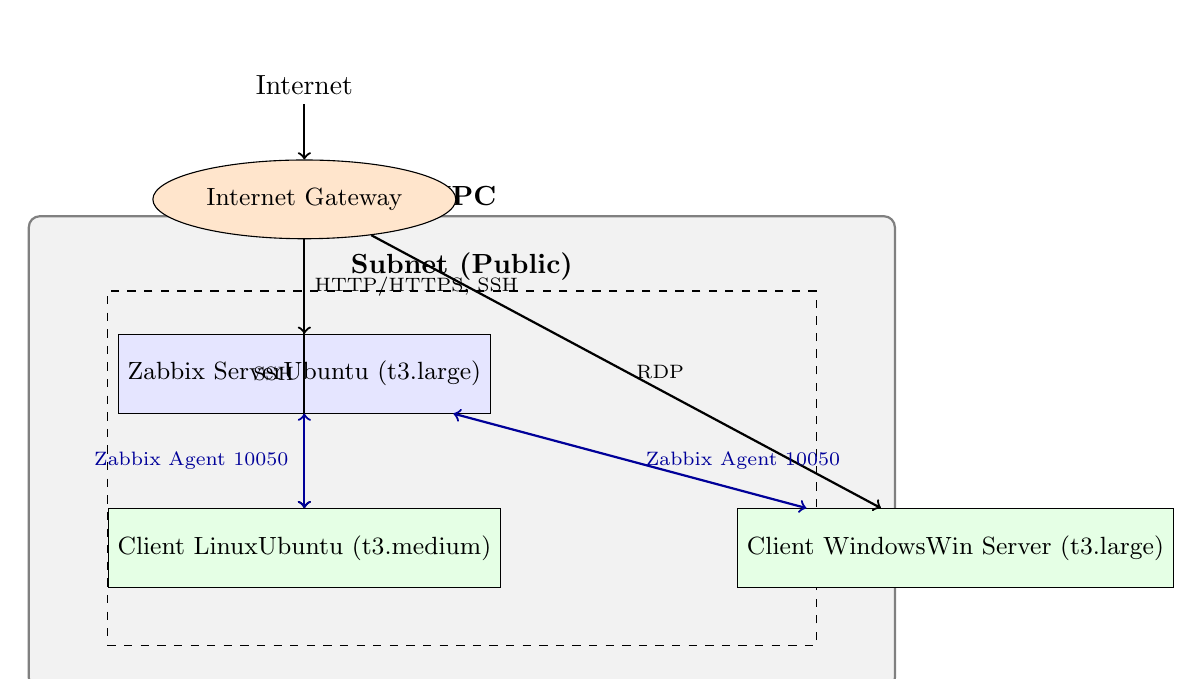
\begin{tikzpicture}[
        server/.style={rectangle, draw, fill=blue!10, minimum width=2.5cm, minimum height=1cm, font=\small},
        client/.style={rectangle, draw, fill=green!10, minimum width=2.5cm, minimum height=1cm, font=\small},
        igw/.style={ellipse, draw, fill=orange!20, minimum width=2cm, minimum height=1cm, font=\small},
        vpc/.style={rounded corners, thick, draw=black!50, fill=gray!10, inner sep=0.5cm}
    ]
    % VPC
    \node[vpc, minimum width=11cm, minimum height=6cm, label=above:{\textbf{VPC}}] (vpc) {};
    % Subnet
    \node[draw, dashed, minimum width=9cm, minimum height=4.5cm, label=above:{\textbf{Subnet (Public)}}] at (0,-0.2) (subnet) {};
    % Zabbix Server
    \node[server] (zabbix) at (-2,1) {Zabbix Server\\Ubuntu (t3.large)};
    % Linux Client
    \node[client, below=1.2cm of zabbix] (linux) {Client Linux\\Ubuntu (t3.medium)};
    % Windows Client
    \node[client, right=3cm of linux] (windows) {Client Windows\\Win Server (t3.large)};
    % IGW
    \node[igw, above=1.2cm of zabbix] (igw) {Internet Gateway};
    % Internet
    \node[draw=none, fill=none, above=0.7cm of igw] (internet) {Internet};
    % Connections
    \draw[->, thick] (igw) -- (zabbix) node[midway, right, font=\scriptsize] {HTTP/HTTPS, SSH};
    \draw[->, thick] (igw) -- (linux) node[midway, left, font=\scriptsize] {SSH};
    \draw[->, thick] (igw) -- (windows) node[midway, right, font=\scriptsize] {RDP};
    \draw[<->, thick, blue!60!black] (zabbix) -- (linux) node[midway, left, font=\scriptsize, xshift=-2pt] {Zabbix Agent 10050};
    \draw[<->, thick, blue!60!black] (zabbix) -- (windows) node[midway, right, font=\scriptsize, xshift=2pt] {Zabbix Agent 10050};
    \draw[->, thick] (internet) -- (igw);
    \end{tikzpicture}
    \caption{Architecture du déploiement Zabbix sur AWS (VPC, Subnet, IGW, Zabbix Server, Clients Linux/Windows)}
\end{figure}
\begin{figure}[H]
    \centering
    \includegraphics[width=0.8\textwidth]{screenshots/zabbix server security groupe .png}
    \caption{Groupe de sécurité Zabbix}
\end{figure}

\noindent
Nous créons un groupe de sécurité pour le serveur Zabbix, autorisant les ports nécessaires (SSH, HTTP, HTTPS, 10051). Cette étape protège l'accès tout en permettant la supervision.
\begin{figure}[H]
    \centering
    \includegraphics[width=0.8\textwidth]{screenshots/linux security groupe .png}
    \caption{Groupe de sécurité Linux}
\end{figure}

\noindent
Un groupe de sécurité spécifique est créé pour l'instance Linux, n'autorisant que les ports requis (SSH, 10050). Cela limite la surface d'attaque et prépare la supervision de l'agent Linux.
\begin{figure}[H]
    \centering
    \includegraphics[width=0.8\textwidth]{screenshots/windows security groupe .png}
    \caption{Groupe de sécurité Windows}
\end{figure}

\noindent
Le groupe de sécurité Windows autorise RDP et le port de l'agent Zabbix. Cette configuration permet la connexion à distance et la supervision du client Windows.
\begin{figure}[H]
    \centering
    \includegraphics[width=0.8\textwidth]{screenshots/associating all security grooups with vpc.png}
    \caption{Association des groupes de sécurité au VPC}
\end{figure}

\noindent
Tous les groupes de sécurité sont associés au VPC, assurant que chaque instance bénéficiera des règles adaptées à son rôle dans l'architecture.

% ===============================
\section{Lancement des instances EC2}
Déploiement des trois instances : Zabbix (Ubuntu), Linux (Ubuntu), Windows (Windows Server). Vérification de leur état de fonctionnement.
\begin{figure}[H]
    \centering
    \includegraphics[width=0.8\textwidth]{screenshots/zabbix instance.png}
    \caption{Instance Zabbix}
\end{figure}

\noindent
Nous lançons l'instance EC2 pour le serveur Zabbix, qui sera le cœur de la supervision. Cette étape précède le déploiement des clients Linux et Windows.
\begin{figure}[H]
    \centering
    \includegraphics[width=0.8\textwidth]{screenshots/linux instance.png}
    \caption{Instance Linux}
\end{figure}

\noindent
L'instance Linux est déployée pour représenter un client supervisé. Elle sera configurée avec l'agent Zabbix dans les étapes suivantes.
\begin{figure}[H]
    \centering
    \includegraphics[width=0.8\textwidth]{screenshots/windows instance .png}
    \caption{Instance Windows}
\end{figure}

\noindent
L'instance Windows complète le parc hybride à superviser. Elle sera également équipée de l'agent Zabbix pour la surveillance.
\begin{figure}[H]
    \centering
    \includegraphics[width=0.8\textwidth]{screenshots/all instances running .png}
    \caption{Instances en fonctionnement}
\end{figure}

\noindent
Les trois instances (Zabbix, Linux, Windows) sont maintenant en fonctionnement, prêtes à être configurées pour la supervision centralisée.

% ===============================
\section{Installation et configuration du serveur Zabbix}
\subsection{Connexion SSH au serveur Zabbix}
Connexion SSH à l’instance Ubuntu Zabbix.
\begin{lstlisting}[language=bash,caption={Connexion SSH}]
ssh -i <cle.pem> ubuntu@<IP-Publique-Zabbix>
\end{lstlisting}
\begin{figure}[H]
    \centering
    \includegraphics[width=0.8\textwidth]{screenshots/connect to ssh zabix server.png}
    \caption{Connexion SSH au serveur Zabbix}
\end{figure}

\noindent
Nous nous connectons en SSH au serveur Zabbix pour procéder à l'installation de Docker et du serveur de supervision.
\begin{figure}[H]
    \centering
    \includegraphics[width=0.8\textwidth]{screenshots/connected to ssh zabix server.png}
    \caption{Connexion établie}
\end{figure}

\noindent
La connexion SSH est établie, nous pouvons maintenant installer les composants nécessaires à l'exécution de Zabbix.

\subsection{Installation de Docker et Docker Compose}
\begin{lstlisting}[language=bash,caption={Installation de Docker et Docker Compose}]
sudo apt update && sudo apt upgrade -y
sudo apt install docker.io -y
sudo systemctl start docker
sudo systemctl enable docker
sudo usermod -aG docker ubuntu
docker --version
sudo apt install docker-compose -y
docker-compose --version
\end{lstlisting}
\begin{figure}[H]
    \centering
    \includegraphics[width=0.8\textwidth]{screenshots/docker has been installed.png}
    \caption{Docker installé}
\end{figure}

\noindent
Docker est installé sur le serveur Zabbix, ce qui permettra de lancer les conteneurs nécessaires à la supervision.
\begin{figure}[H]
    \centering
    \includegraphics[width=0.8\textwidth]{screenshots/docker compose has been installed.png}
    \caption{Docker Compose installé}
\end{figure}

\noindent
Docker Compose est ajouté pour faciliter la gestion et l'orchestration des conteneurs Zabbix et de la base de données.

\subsection{Déploiement de Zabbix via Docker Compose}
Création du fichier docker-compose.yml et lancement des conteneurs.
\begin{lstlisting}[language=bash,caption={Lancement de Zabbix avec Docker Compose}]
# Créer docker-compose.yml puis :
docker-compose up -d
docker ps
\end{lstlisting}
\begin{figure}[H]
    \centering
    \includegraphics[width=0.8\textwidth]{screenshots/docker compose file.png}
    \caption{Fichier docker-compose.yml}
\end{figure}

\noindent
Le fichier docker-compose.yml est créé pour décrire la configuration des services Zabbix, Web et base de données. Il sera utilisé pour lancer l'ensemble de la stack.
\begin{figure}[H]
    \centering
    \includegraphics[width=0.8\textwidth]{screenshots/contrainers running.png}
    \caption{Conteneurs en fonctionnement}
\end{figure}

\noindent
Après exécution de Docker Compose, tous les conteneurs nécessaires à Zabbix sont en fonctionnement. Nous pouvons maintenant accéder à l'interface web.

\subsection{Accès à l’interface Zabbix}
Connexion à l’interface web de Zabbix.
\begin{figure}[H]
    \centering
    \includegraphics[width=0.8\textwidth]{screenshots/zabbix interface login accessible.png}
    \caption{Page de connexion Zabbix}
\end{figure}

\noindent
L'interface de connexion Zabbix est accessible via le navigateur. Nous pouvons nous connecter pour commencer la configuration de la supervision.
\begin{figure}[H]
    \centering
    \includegraphics[width=0.8\textwidth]{screenshots/first look into zabbix interface.png}
    \caption{Première vue de l’interface Zabbix}
\end{figure}

\noindent
Première connexion à l'interface Zabbix, où nous allons ajouter les hôtes à superviser et configurer les agents.

% ===============================
\section{Configuration des clients}
\subsection{Client Linux}
Connexion SSH à l’instance Linux, installation et configuration de l’agent Zabbix.
\begin{lstlisting}[language=bash,caption={Installation et configuration de l’agent Zabbix sur Linux}]
wget https://repo.zabbix.com/zabbix/6.4/ubuntu/pool/main/z/zabbix-release/zabbix-release_6.4-1+ubuntu22.04_all.deb
sudo dpkg -i zabbix-release_6.4-1+ubuntu22.04_all.deb
sudo apt update
sudo apt install zabbix-agent -y
sudo nano /etc/zabbix/zabbix_agentd.conf
# Modifier Server, ServerActive, Hostname
sudo systemctl restart zabbix-agent
sudo systemctl enable zabbix-agent
sudo systemctl status zabbix-agent
\end{lstlisting}
\begin{figure}[H]
    \centering
    \includegraphics[width=0.8\textwidth]{screenshots/connected to linux ssh.png}
    \caption{Connexion SSH à Linux}
\end{figure}

\noindent
Connexion SSH à l'instance Linux pour installer et configurer l'agent Zabbix, étape préalable à l'ajout de la machine dans l'interface de supervision.
\begin{figure}[H]
    \centering
    \includegraphics[width=0.8\textwidth]{screenshots/configured zabbix agent.png}
    \caption{Configuration de l’agent Zabbix}
\end{figure}

\noindent
L'agent Zabbix est configuré sur la machine Linux pour pointer vers le serveur Zabbix. Cette configuration permet la remontée des métriques.
\begin{figure}[H]
    \centering
    \includegraphics[width=0.8\textwidth]{screenshots/zabbix agent working.png}
    \caption{Agent Zabbix actif}
\end{figure}

\noindent
Après démarrage du service, l'agent Zabbix fonctionne correctement sur Linux. Nous pouvons maintenant l'ajouter comme hôte dans Zabbix.

\subsection{Client Windows}
Connexion via RDP, installation et configuration de l’agent Zabbix.
\begin{figure}[H]
    \centering
    \includegraphics[width=0.8\textwidth]{screenshots/connected to windows instance via rdp .png}
    \caption{Connexion RDP à Windows}
\end{figure}

\noindent
Connexion à l'instance Windows via RDP pour installer l'agent Zabbix, étape similaire à celle réalisée sur Linux.
\begin{figure}[H]
    \centering
    \includegraphics[width=0.8\textwidth]{screenshots/installed zabbix in windows .png}
    \caption{Installation de Zabbix sur Windows}
\end{figure}

\noindent
L'agent Zabbix est installé sur Windows, prêt à être configuré pour communiquer avec le serveur de supervision.
\begin{figure}[H]
    \centering
    \includegraphics[width=0.8\textwidth]{screenshots/configured zabbix agent.png}
    \caption{Configuration de l’agent Zabbix sur Windows}
\end{figure}

\noindent
L'agent Zabbix sur Windows est configuré pour pointer vers le serveur Zabbix, permettant la collecte des métriques système.

% ===============================
\section{Ajout des hôtes dans Zabbix}
Ajout des clients Linux et Windows dans l’interface Zabbix, vérification de la connexion des agents.
\begin{figure}[H]
    \centering
    \includegraphics[width=0.8\textwidth]{screenshots/ADDED AGENTS TO ZABBIX INTERFACE.png}
    \caption{Ajout des agents à l’interface Zabbix}
\end{figure}

\noindent
Les agents Linux et Windows sont ajoutés dans l'interface Zabbix. On vérifie leur statut et la bonne remontée des données.
\begin{figure}[H]
    \centering
    \includegraphics[width=0.8\textwidth]{screenshots/zabbix agent working.png}
    \caption{Agent Zabbix opérationnel}
\end{figure}

\noindent
Le statut opérationnel des agents est confirmé dans l'interface, attestant du bon fonctionnement de la supervision sur les deux clients.

% ===============================
\section{Supervision et alertes}
Visualisation des données en temps réel (CPU, RAM, etc.), test d’alerte et analyse graphique des performances des clients.

\begin{figure}[H]
    \centering
    \includegraphics[width=0.8\textwidth]{screenshots/dashboard.png}
    \caption{Tableau de bord Zabbix}
\end{figure}
\noindent
Le tableau de bord Zabbix présente une vue d'ensemble de l'état du parc supervisé. On y retrouve les alertes, les performances et le statut des hôtes surveillés.

\begin{figure}[H]
    \centering
    \includegraphics[width=0.8\textwidth]{screenshots/client_ubunto_monitoring.png}
    \caption{Surveillance du client Ubuntu}
\end{figure}
\noindent
Ce graphique montre la supervision en temps réel du client Ubuntu, avec des métriques telles que l'utilisation CPU, la mémoire et le statut de l'agent. Cela permet de détecter rapidement toute anomalie sur le serveur Linux.

\begin{figure}[H]
    \centering
    \includegraphics[width=0.8\textwidth]{screenshots/client_windows_monitoring.png}
    \caption{Surveillance du client Windows}
\end{figure}
\noindent
La surveillance du client Windows affiche les indicateurs de performance et le statut de l'agent Zabbix. On peut ainsi suivre l'activité du serveur Windows et réagir en cas d'alerte ou de problème.

\noindent
Grâce à ces graphiques, l'administrateur dispose d'une vision claire et synthétique de l'état du parc hybride, facilitant la gestion proactive des incidents et l'optimisation des ressources.

% ===============================
\section{Conclusion}
Ce projet a permis de mettre en œuvre une infrastructure de supervision centralisée sur AWS, adaptée à un parc hybride Linux et Windows. Toutes les étapes, de la création du réseau à la configuration des agents et à la visualisation des métriques, ont été réalisées avec succès.

Parmi les difficultés rencontrées, la configuration fine des groupes de sécurité et l'intégration des agents sur Windows ont nécessité une attention particulière. L'utilisation de Docker et Docker Compose a grandement simplifié le déploiement du serveur Zabbix.

La supervision graphique et la remontée des alertes permettent désormais une gestion proactive des incidents et une optimisation continue des ressources. Ce projet est valorisé par la documentation complète, les captures d'écran et le dépôt GitHub associé.

\end{document}